\section{Аналитическая часть}

\subsection{Постановка задачи}

Сравнительный анализ геномов ставит задачу обнаружения гомологичных участков -- подпоследовательностей геномов, указывающих на общее происхождение\cite{1_hardison2003comparative} организмов-носителей. Как правило, гомологичность выводится из избыточной схожести строк\cite{2_pearson2013introduction}. В задаче определения схожести подпоследовательностей геномов необходимо учитывать случайные мутации, наблюдаемые при репликации, а также ошибки секвенирования. Таким образом, сравнительный анализ предполагает как детерминированый, так и вероятностный аспекты, в силу того, что геномная информация содержит вариации как в рамках одного вида\cite{3_barrick2009genome,4_barnetson2008classification}, так и между видами. Более того, вероятности возникновения точечных мутаций различны для разных типов точечных мутаций\cite{5_zhu2017statistical} и для разных видов\cite{5_zhu2017statistical}, а также могут зависеть от соседних подпоследовательностей\cite{5_zhu2017statistical}.

\subsection{Классификация методов сравнительного анализа геномов}

Для сравнения геномов активно применяются методы, основанные на поиске выравниваний строк\cite{6_altschul1990basic,7_altschul1997gapped,8_thompson1994clustal}. Поиск выравниваний позволяет обнаружить гомологичные участки, а также оценить степень схожести геномных последовательностей. Однако, показано, что задача поиска множественного локального выравнивания, а также задача поиска локального выравнивания в случае последовательностей с повторяющимися подстроками, являются NP-трудными\cite{9_perrey1996fast}. В качестве альтернативных подходов, не требующих поиска выравнивания, предложены следующие методы: статистический анализ строк\cite{10_sarkar2021determination,11_bernard2018k} и теоретико-графовые методы\cite{12_aguero2020graph,13_minkin2017twopaco}. Статистический анализ геномов позволяет оценить степень схожести последовательностей, но не локализовать гомологичные подструктуры. Показано, что использование графовых структур, в частности – графа де Брюйна\cite{13_minkin2017twopaco}, позволяет решить задачу обнаружения гомологичных участков геномов без выполнения трудоемкого поиска выравниваний. На рисунке \ref{fig:classif} продемонстрирована классификация методов сравнительного анализа геномов.

\begin{figure}[htbp]
	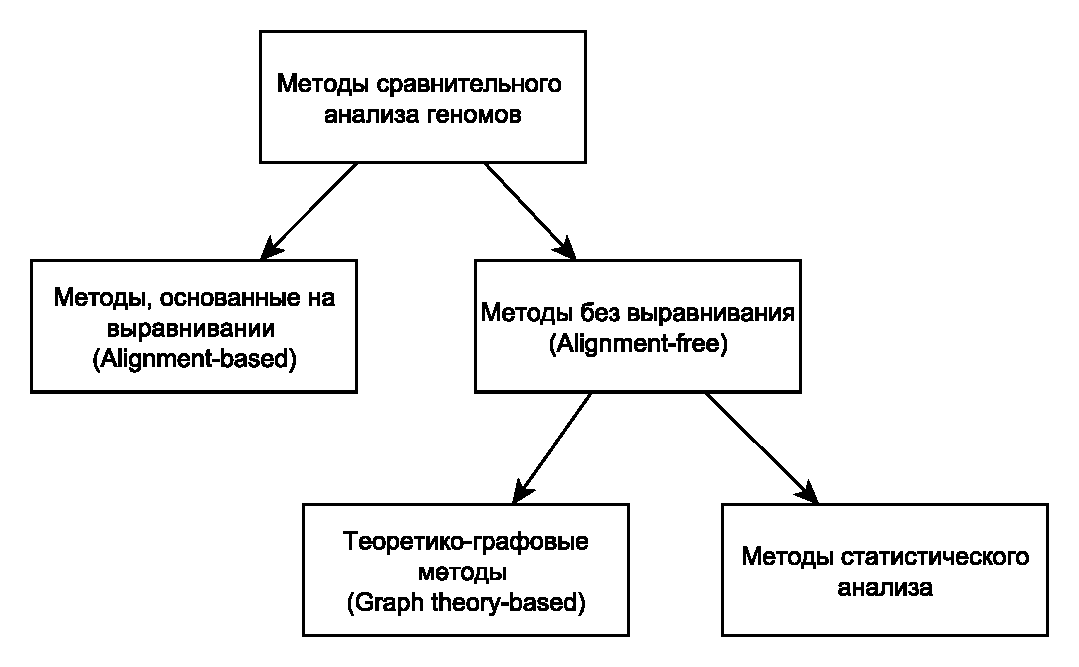
\includegraphics[width=\textwidth]{img/classif.pdf}
	\caption{Классификация методов сравнительного анализа геномов.}
	\label{fig:classif}
\end{figure}

\subsection{Граф де Брюйна}

Граф де Брюйна $ B\left(\Sigma,k\right) $, построенный для алфавита $ \Sigma  $ и параметра $ k $, это ориентированный граф $ G\left(V,E\right) $, где $ V $ это множество всех слов длины $ k $ в алфавите $ \Sigma $, называемых $ k$-мерами, и $ \left(u,v\right)\in E\leftrightarrow suffix\left(u\right)=prefix\left(v\right) $. Формальное опредление графа де Брюйна приведено в \ref{eq:dbg_def}. Пример графа де Брюйна, построенного для бинарного алфавита $ \Sigma_{\{0,1\}}=\{0,1\} $ и параметра $ k=3 $ показан на рисунке \ref{fig:dbg_ex}.

\begin{equation}
	\begin{split}
		B\left(\Sigma,k\right)=G\left(V,E\right): V=\Sigma^k, \\
		\left(u,v\right)\in E\leftrightarrow suffix\left(u\right)=prefix\left(v\right)
	\end{split}
	\label{eq:dbg_def}
\end{equation}


\begin{figure}[htbp]
	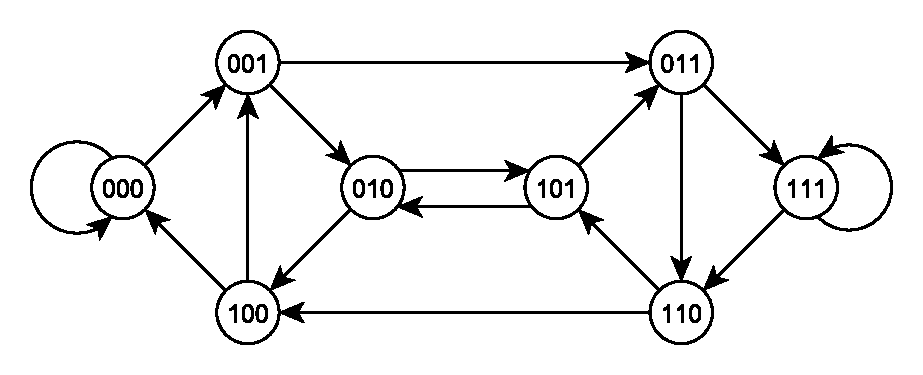
\includegraphics[width=\textwidth]{img/dbg_ex.pdf}
	\caption{Граф де Брюйна для $ \Sigma_{\{0,1\}}=\{0,1\} $ и $ k=3 $.}
	\label{fig:dbg_ex}
\end{figure}

\subsection{Анализ пан-генома}

TODO: пан-геном/мульти-геном более репрезентативный, чем геном, поэтому есть смысл конструировать базу для хранения пангеномов, нежели геномов. 

TODO описать: Кроме того, было показано, что дискретные последовательности (символов?), такие как строка ДНК, могут быть представлены в виде Марковской цепи\cite{17_heath2021computing}.

\subsection{Марковская цепь}

Пусть $ \{X^{\left(1\right)},X^{\left(2\right)},\ldots\} $ -- последовательность случайных переменных, принимающих значения из некоторого конечного множества $ M $. Переменная $ X^{\left(i\right)} $ рассматривается как состояние некоторой системы в момент времени $ i > 0 $. Тогда последовательность $ \{X^{\left(1\right)},X^{\left(2\right)},\ldots\} $ представляет собой случайный процесс, а множество $ M $ называется $ пространством\ состояний $ процесса. Процесс $ \{X^{\left(1\right)},X^{\left(2\right)},\ldots\} $ называется марковской цепью\cite{14_billingsley1961statistical} если выполняется условие, представленное в уравнении \ref{eq:mc_def}.

\begin{equation}
	\begin{split}
		P\{X^{\left(i+1\right)}=x_{i+1}\ \vert \ X^{\left(i\right)}=x_i,X^{\left(i-1\right)}=x_{i-1},\ldots, \\
		X^{\left(1\right)}=x_1\}=P\{X^{\left(i+1\right)}=x_{i+1}\ \vert \ X^{\left(i\right)}=x_i\}
	\end{split}
	\label{eq:mc_def}
\end{equation}

то есть, условная вероятность $ P\{X^{\left(i+1\right)}=x_{i+1}\ \vert \ X^{\left(i\right)}=x_i\} $ не зависит от значений переменных $ X^{\left(j\right)} $ для $ j<i-1 $. Для пространства состояний $ M $, вероятность перехода $ p_{uv} $ -- это вероятность того, что процесс, находящийся в текущий момент времени в состоянии  $ v \in M $, выполнит переход в состояние $ u \in M $. Формальное определение вероятности перехода $ p_{uv} $ приведено в \ref{eq:mc_note1}. Исходная вероятность $ p_u $ -- это вероятность наблюдения процесса в состоянии $ u \in M $ в начальный момент времени.

\begin{equation}
	p_{uv}=P\{X^{\left(i+1\right)}=v\ \vert \ X^{\left(i\right)}=u\}
	\label{eq:mc_note1}
\end{equation}

Пусть для некоторый процесс посетил последовательность из $ n $ состояний $ S=\left(s_1,s_2,\ldots,s_n\right) $, и пусть $ f_{uv} $ -- число $ i\in\left[1,n\right) $, таких что: $ s_i=u,\ s_{i+1}=v $. То есть $ f_{uv} $ -- это количество раз, когда процесс выполнил переход из состояния $ u $ в состояние $ v $. Вероятность наблюдения последовательности состояний $ S=\left(s_1,s_2,\ldots,s_n\right) $ представлена в уравнении \ref{eq:mc_note2}.

\begin{equation}
	p_S=p_{s_1}\cdot p_{s_1s_2}\cdot\ldots\cdot p_{s_{n-1}s_n}=p_{s_1}\cdot\prod_{u,v} p_{uv}^{\ f_{uv}}
	\label{eq:mc_note2}
\end{equation}

Марковская цепь может быть представлена в виде ориентированного графа $ G\left(V,E\right) $, где $ V $ -- пространство состояний процесса, и $ \left(u,v\right)\in E\leftrightarrow p_{uv}>0 $, каждому ребру $ \left(u,v\right)\in E $ в соответствие поставлено значение $ p_{uv} $, называемое весом ребра. Пример графового представление цепи Маркова продемонтрирован на рисунке \ref{fig:mc_ex}.

\begin{figure}[htbp]
	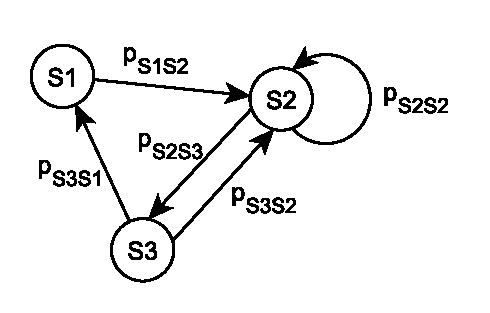
\includegraphics[width=0.8\textwidth]{img/mc_ex.pdf}
	\caption{Графовое представление цепи Маркова.}
	\label{fig:mc_ex}
\end{figure}

Таким образом, некоторая последовательность состояний процесса $ S=\left(s_1,s_2,\ldots,s_n\right) $ представляет собой путь в графе, описывающем Марковскую цепь для этого процесса; вероятность $ p_S $ наблюдения последовательности состояний $ S $ может быть посчитана как произведение весов ребер, составляющих этот путь. Заметим, что есть вероятности перехода для процесса неизвестны, встает вопрос о выводе вероятностей из эмпирических данных.

\subsection{Графовые СУБД}
Данные в графовых хранилищах представлены наборами узлов и ребер, где узлы описывают некоторые сущности предметной области, а ребра – связи между ними. Хранение связей в явном виде позволяет избежать необходимости выполнения дорогостоящей операции соединения, характерной для реляционных баз данных. Кроме того, сетевая модель данных, реализованная в графовых хранилищах, допускает динамическое определение новых типов связей благодаря отсутствию схем отношений. Таким образом, в случаях, когда связи между сущностями несут не меньше информации, чем сами сущности, или могут быть динамически изменены, графовые базы предлагают более эффективный\cite{20_batra2012comparative,21_medhi2017relational} подход к хранению и обработке данных по сравнению с реляционными решениями. Сопоставляя представление геномной информации в виде графа, с данными критериями, можно сделать вывод о возможности использования графовой базы данных при решении задач сравнительной геномики\cite{22_miller2013graph}.

\pagebreak